\documentclass[12pt]{article}

% Encoding and fonts
\usepackage[utf8]{inputenc}
\usepackage[T1]{fontenc}
\usepackage{lmodern}

% Page setup
\usepackage[margin=1in]{geometry}
\usepackage{setspace}
\doublespacing

% Typography
\usepackage{microtype}

% Math
\usepackage{amsmath,amssymb}

% Graphics
\usepackage{graphicx}
\usepackage{float}
\usepackage{subcaption}

% Tables
\usepackage{booktabs}
\usepackage{array}
\usepackage{multirow}
\usepackage{threeparttable}

% Bibliography
\usepackage{natbib}
\bibliographystyle{aer}

% Hyperlinks
\usepackage{hyperref}
\hypersetup{colorlinks=true, linkcolor=blue, citecolor=blue, urlcolor=blue}
\usepackage[nameinlink,noabbrev]{cleveref}

% Timing
\newcommand{\apepcurrenttime}{---}
\newcommand{\apepcumulativetime}{---}

% Captions
\usepackage{caption}
\captionsetup{font=small,labelfont=bf}

% Section formatting
\usepackage{titlesec}
\titleformat{\section}{\large\bfseries}{\thesection.}{0.5em}{}
\titleformat{\subsection}{\normalsize\bfseries}{\thesubsection}{0.5em}{}

\title{Demand Recessions Scar, Supply Recessions Don't:\\ Evidence from State Labor Markets\footnote{This paper is a revision of APEP-0238. See \url{https://github.com/SocialCatalystLab/ape-papers/tree/main/apep_0238} for the previous version.}}
\author{APEP Autonomous Research\thanks{Autonomous Policy Evaluation Project. Correspondence: scl@econ.uzh.ch} \and @SocialCatalystLab \and @dyanag}
\date{\today}

\begin{document}

\maketitle

\begin{abstract}
\noindent
Why did the U.S.\ labor market recover slowly after the Great Recession but rapidly after COVID-19? I compare the same fifty state labor markets across the two episodes, using within-episode cross-state exposure measures---housing boom intensity for the Great Recession and Bartik industry exposure for COVID---and summarize long-run outcomes with pre-specified post-recession employment averages. Three findings emerge. First, states more exposed to the housing bust suffered persistent employment shortfalls years after the Great Recession. Second, states more exposed to COVID did not experience comparable long-run deficits once the pandemic shock passed. Third, evidence on unemployment persistence, long-term joblessness, and temporary layoffs points to the same mechanism: recessions leave lasting scars when they generate prolonged nonemployment, not simply when they destroy many jobs on impact.
\end{abstract}

\vspace{1em}
\noindent\textbf{JEL Codes:} E24, E32, J63, J64 \\
\noindent\textbf{Keywords:} hysteresis, labor market scarring, duration trap, recessions, Great Recession, COVID-19

\newpage

%% ═══════════════════════════════════════════════════════════
\section{Introduction}
\label{sec:introduction}
%% ═══════════════════════════════════════════════════════════

The Great Recession and the COVID-19 recession produced the two largest U.S.\ employment collapses since the Great Depression, but their recoveries were radically different. After 2008, employment fell by about 6 percent and took roughly six years to recover. In 2020, employment fell by nearly 15 percent and returned within two. This paper asks why. The central hypothesis is that labor markets are scarred less by the size of the initial drop than by what happens afterward: when a downturn pushes workers into prolonged nonemployment, skill loss, detachment, and labor-force exit can outlast the shock itself.

To study that question, I compare the same fifty state labor markets across both episodes using within-episode variation in recession exposure: pre-crisis housing booms for the Great Recession \citep{mian2014explains} and Bartik industry exposure for COVID \citep{goldsmith2020bartik}. I estimate pre-specified long-run employment outcomes---average employment growth over months 48--120 after the Great Recession and 24--48 after COVID---and then trace the intermediate dynamics with local projections and duration-based mechanism evidence. The cross-episode contrast is not a pure estimate of demand versus supply shocks, since policy responses, temporary layoffs, and sectoral composition also differed. But it provides a disciplined comparison of two severe downturns and asks a sharp question: which recessions leave lasting employment gaps, and which do not?

Three findings emerge. First, states more exposed to the housing bust suffered persistent relative employment deficits: the long-run scarring coefficient is $-0.057$ (permutation $p \approx 0.13$), with statistically significant effects at medium horizons ($h = 3$, 6, 12 months). Second, states more exposed to COVID show no comparable long-run deficits; the exposure gradient converges to zero within 18 months. Third, the persistence gap is tightly linked to unemployment duration. National data show that the Great Recession generated unprecedented long-term unemployment (45\% of the unemployed at 27+ weeks), while COVID produced mainly temporary layoffs with rapid recall. At the state level, controlling for unemployment persistence at $h = 24$ months absorbs 38\% of the Great Recession scarring coefficient; at $h = 48$, it absorbs 77\%. The mechanism is the duration trap: demand downturns that generate prolonged nonemployment scar; temporary disruptions that preserve matches do not.

This paper's central contribution is to show that long-run labor-market scarring is tied less to the depth of the initial employment collapse than to whether a recession turns job loss into prolonged nonemployment. This advances the hysteresis literature \citep{blanchard1986hysteresis, cerra2008growth, cerra2023hysteresis} by identifying the duration trap as the operative mechanism, contributes to the study of local labor market adjustment \citep{blanchard1992regional, autor2013china, yagan2019employment} by showing that recovery speed depends on shock type, and connects the COVID recession literature \citep{chetty2020real, cajner2020us, autor2022paycheck} to the broader question of when recessions leave permanent scars.


%% ═══════════════════════════════════════════════════════════
%% ═══════════════════════════════════════════════════════════
\section{Episodes, Design, and Estimand}
\label{sec:design}
%% ═══════════════════════════════════════════════════════════

\subsection{Why These Two Episodes}

The Great Recession and COVID-19 provide a near-ideal laboratory. Both were severe, affected all 50 states, and featured substantial cross-state variation in severity driven by well-understood sources. The Great Recession was a demand collapse: falling home values eroded household wealth, depressing spending and hiring for years \citep{mian2014explains}. The share of workers unemployed for 27+ weeks rose from 17\% to 45\%, and mean unemployment duration peaked at 39 weeks \citep{kroft2016long}. COVID was a supply disruption: an abrupt, sectoral shutdown that generated mass temporary layoffs but preserved employer-employee matches. Median unemployment duration peaked at only 10 weeks, and 78\% of the unemployed in April 2020 reported their layoff as temporary \citep{fujita2017recall, cajner2020us}.

The critical difference for hysteresis lies in what happened \textit{during} each downturn. The Great Recession's demand collapse was not a temporary disruption---it was a sustained reduction in the willingness to spend. Firms permanently closed establishments and did not rehire even as conditions slowly improved. The policy response arrived with a lag: the Federal Reserve reached the zero lower bound by December 2008, and ARRA took effect in February 2009, by which time millions had already entered long unemployment spells \citep{elsby2010labor}. By contrast, the COVID shock preserved employer-employee matches. The PPP provided \$800 billion in forgivable payroll loans, directly subsidizing match preservation \citep{autor2022paycheck}. Enhanced unemployment insurance maintained household income \citep{ganong2020us}. Workers were furloughed rather than permanently separated. Consumer spending on durable goods actually \textit{increased} during 2020 \citep{guerrieri2022macroeconomic}.

The episodes also differed in policy timing, monetary conditions, and labor market institutions. I therefore interpret the cross-episode contrast as evidence on the full treatment package---shock type, policy, and sectoral dynamics---not as a pure causal estimate of demand versus supply shocks. The within-episode variation (housing exposure for the Great Recession, Bartik industry composition for COVID) provides the credible quasi-experimental variation; the comparison across episodes provides the interpretive framework.

The duration-trap hypothesis predicts three empirical patterns. First, Great Recession exposure should produce persistent negative employment effects at horizons of 48 months or more. Second, COVID exposure effects should converge to zero within 18--24 months. Third, the persistence gap should operate through unemployment duration---controlling for duration-trap measures should attenuate the Great Recession scarring coefficient. Workers who remain unemployed beyond roughly six to twelve months face compounding disadvantages: skills depreciate, employer networks atrophy, and stigma reduces callback rates \citep{kroft2016long}. Some exit the labor force entirely. Supply recessions short-circuit this process because temporary separations enable rapid recall before human capital depreciates.

\subsection{Exposure Measures and Identification}

\textit{Great Recession: housing price boom.} I measure state-level exposure to the Great Recession using the log change in the FHFA house price index between 2003Q1 and 2006Q4, following \citet{mian2014explains} and \citet{charles2016masking}. States where the bubble inflated most experienced the largest demand collapse when it burst. The identifying assumption is that cross-state variation in the housing boom captures cross-state variation in demand collapse severity, conditional on pre-recession employment growth and census region. I instrument the housing boom with the \citet{saiz2010geographic} housing supply elasticity (first-stage $F = 11.4$) as supporting evidence for the demand channel.

\textit{COVID: Bartik shock.} I construct a shift-share exposure measure based on pre-pandemic (2019) industry employment shares interacted with national leave-one-out industry-level employment changes between February and April 2020 \citep{goldsmith2020bartik, borusyak2022quasi}. The instrument exploits the sectoral incidence of COVID: contact-intensive industries (leisure, hospitality) contracted sharply regardless of geography. The raw Bartik values are negative for all states (mean $= -0.137$); I standardize to mean zero and unit variance for regression. Under this convention, states with more negative standardized values experienced larger COVID shocks. A positive LP coefficient indicates that less-exposed states (higher standardized values) had higher employment---equivalently, that COVID exposure reduced employment.

\textit{Controls.} All specifications include log pre-recession employment at the peak, pre-recession employment growth, and census region indicators. I show robustness to richer control sets (construction and manufacturing employment shares) in Section~\ref{sec:robustness}.

\textit{Threats to validity.} Three concerns deserve discussion. First, \textit{endogeneity of housing prices}: the literature has established that the housing boom was driven primarily by credit supply expansion interacting with geographic supply constraints, not by local labor demand \citep{mian2013household}. The relevant variation is in the \textit{boom}---before 2006---while outcomes are measured \textit{after} the bust. Second, \textit{migration}: if damaged workers move elsewhere, state-level data hides their hardship behind population reshuffling. I address this by noting that \citet{yagan2019employment} shows individual-level scarring persists even after controlling for migration, and \citet{dao2017regional} document declining interstate mobility. Third, \textit{general equilibrium}: cross-state LP estimates capture \textit{relative} scarring. If spillovers attenuate cross-state differences, the LP coefficients understate aggregate scarring---a conservative bias for the paper's central claim.

\subsection{Data}

I use state-level labor market data from the Bureau of Labor Statistics, covering all 50 states at monthly frequency from 2000 to 2024. The primary data sources are the Current Employment Statistics (CES) for nonfarm payroll employment, the Local Area Unemployment Statistics (LAUS) for unemployment rates and labor force participation rates, and the Federal Housing Finance Agency (FHFA) for state-level house price indices. All series are accessed through the Federal Reserve Economic Data (FRED) API.

For the mechanism analysis, I supplement these aggregate series with CPS-derived variables. National-level long-term unemployment share (workers unemployed 27+ weeks as a fraction of total unemployed) and temporary layoff share come from published BLS series. State-level unemployment rate responses serve as proxies for the duration-trap mechanism, capturing whether cross-state employment differentials deepen over time (duration trap) or resolve (recall).

Industry employment by major supersector (10 industries) from the CES program provides the building blocks for the Bartik instrument construction. 
\Cref{tab:summary} reports summary statistics. The housing price boom averages 0.30 log points with substantial cross-state variation (SD = 0.15). The COVID Bartik shock is an order of magnitude smaller in cross-state variation (SD = 0.01), reflecting the more uniform sectoral incidence of the pandemic. The analysis sample is a balanced panel of 50 states $\times$ 294 months $= 14{,}700$ state-month observations.

\begin{table}[H]
\centering
\caption{Summary Statistics}
\begin{threeparttable}
\begin{tabular}{lrrrrr}
\toprule
Variable & Mean & Std. Dev. & Min & Max & N \\
\midrule
Housing price boom (log, 2003--2006) & 0.303 & 0.147 & 0.065 & 0.615 & 50 \\
COVID Bartik shock (raw) & -0.1368 & 0.0100 & -0.1902 & -0.1263 & 50 \\
Saiz supply elasticity & 2.06 & 0.74 & 0.70 & 3.50 & 50 \\
\bottomrule
\end{tabular}
\begin{tablenotes}[flushleft]
\small
\item \textit{Notes:} Housing price boom is the log change in the FHFA state-level house price index from 2003Q1 to 2006Q4. COVID Bartik shock is constructed using pre-pandemic (2019) industry employment shares weighted by leave-one-out national industry employment changes (Feb--Apr 2020). Saiz supply elasticity is from \citet{saiz2010geographic}, measuring geographic constraints on housing supply.
\end{tablenotes}
\end{threeparttable}
\label{tab:summary}
\end{table}


\subsection{Single Estimand}

The primary estimand is the average log employment change over a post-recovery horizon window. For the Great Recession, I use months 48--120 post-peak (December 2007); for COVID, I use months 24--48 post-peak (February 2020), chosen to balance sufficient post-recovery observation time with data availability through June 2024. The windows differ because the Great Recession occurred earlier and permits a longer follow-up; this is an inherent feature of comparing a historical episode with a recent one. The single-regression approach avoids the multiple-testing problems inherent in horizon-by-horizon local projections while preserving the core question: does recession exposure predict persistent employment deficits? For each state $s$:
\begin{equation}
\bar{y}_s = \frac{1}{|\mathcal{H}|} \sum_{h \in \mathcal{H}} \left[ \ln(E_{s,t_0+h}) - \ln(E_{s,t_0}) \right],
\end{equation}
where $\mathcal{H} = \{48, 51, 54, \ldots, 120\}$ is the set of post-recovery horizons at 3-month intervals, and $t_0$ is the recession peak. The headline regression is:
\begin{equation}
\bar{y}_s = \alpha + \pi \cdot Z_s + X_s'\phi + \varepsilon_s,
\label{eq:main}
\end{equation}
where $Z_s$ is the recession exposure measure and $X_s$ is the control vector. A negative $\hat{\pi}$ for the Great Recession and a near-zero $\hat{\pi}$ for COVID would confirm the scarring asymmetry.

The window is justified on economic grounds: 48 months is sufficient for cyclical recovery to have completed; 120 months is the sample limit for the Great Recession. I show robustness to alternative windows (36--96, 48--96, 60--120) in Section~\ref{sec:robustness}.

I also report dynamic local projection impulse response functions for transparency, following \citet{jorda2005estimation}. For the Great Recession, horizons extend to $h = 120$ months; for COVID, I use horizons through $h = 48$ (February 2020 through February 2024). For each horizon:
\begin{equation}
\Delta y_{s,h} = \alpha_h + \pi_h \cdot Z_s + X_s'\phi_h + \varepsilon_{s,h},
\label{eq:lp}
\end{equation}
where $\Delta y_{s,h} = \ln(E_{s,t_0+h}) - \ln(E_{s,t_0})$. These are supporting evidence---the reader can see the full dynamic path---but the headline inference rests on the single estimand.

\textit{Inference.} Permutation $p$-values (2,000 random reassignments of the exposure measure) are the primary inference device, providing exact finite-sample validity without distributional assumptions in a 50-state cross-section. HC1 robust standard errors are reported for reference. With 50 observations, asymptotic approximations may be unreliable; permutation inference avoids this concern entirely.


%% ═══════════════════════════════════════════════════════════
\section{Main Results}
\label{sec:results}
%% ═══════════════════════════════════════════════════════════

\subsection{Great Recession: Persistent Scarring}

\Cref{tab:main} reports the central result. States with larger housing booms suffered persistent employment deficits: the coefficient on HPI boom in the single-estimand regression is $-0.057$, indicating that a one-unit increase in the log housing boom is associated with 5.7 percent lower employment averaged over months 48--120. The coefficient is imprecise in the 50-state cross-section (permutation $p \approx 0.13$), reflecting the well-known power limitations of state-level designs. However, the horizon-by-horizon LP estimates are statistically significant at $h = 3$, $h = 6$, and $h = 12$ under permutation inference (see Appendix~\ref{app:dynamic}), and the horse race and IV specifications support the demand channel. In states where the bubble burst hardest, roughly one in every hundred workers was still missing from payrolls four to ten years later.

\begin{table}[H]
\centering
\caption{Long-Run Employment Response to Recession Exposure}
\begin{threeparttable}
\begin{tabular}{lcc}
\toprule
& Great Recession & COVID-19 \\
& (avg months 48--120) & (avg months 24--48) \\
\midrule
Exposure & $-0.0567$ & $0.0029$ \\
& (0.0467) & (0.0026) \\
$R^2$ & 0.146 & 0.737 \\
\midrule
$N$ & 50 & 50 \\
\bottomrule
\end{tabular}
\begin{tablenotes}[flushleft]
\small
\item \textit{Notes:} Each column reports the coefficient from a cross-state regression of average log employment change over the specified horizon window on recession exposure. Great Recession exposure is the 2003--2006 housing price boom (log change). COVID exposure is the standardized Bartik shock (mean zero, unit variance). Controls: log pre-recession employment, pre-recession employment growth, census region indicators. Robust (HC1) standard errors in parentheses. $^{*}$~$p<0.10$, $^{**}$~$p<0.05$, $^{***}$~$p<0.01$.
\end{tablenotes}
\end{threeparttable}
\label{tab:main}
\end{table}


\Cref{fig:main_scatter} displays the relationship visually. Panel~A shows a clear negative gradient: states with larger housing booms experienced worse long-run employment outcomes. The relationship is not driven by outliers.

\begin{figure}[H]
\centering
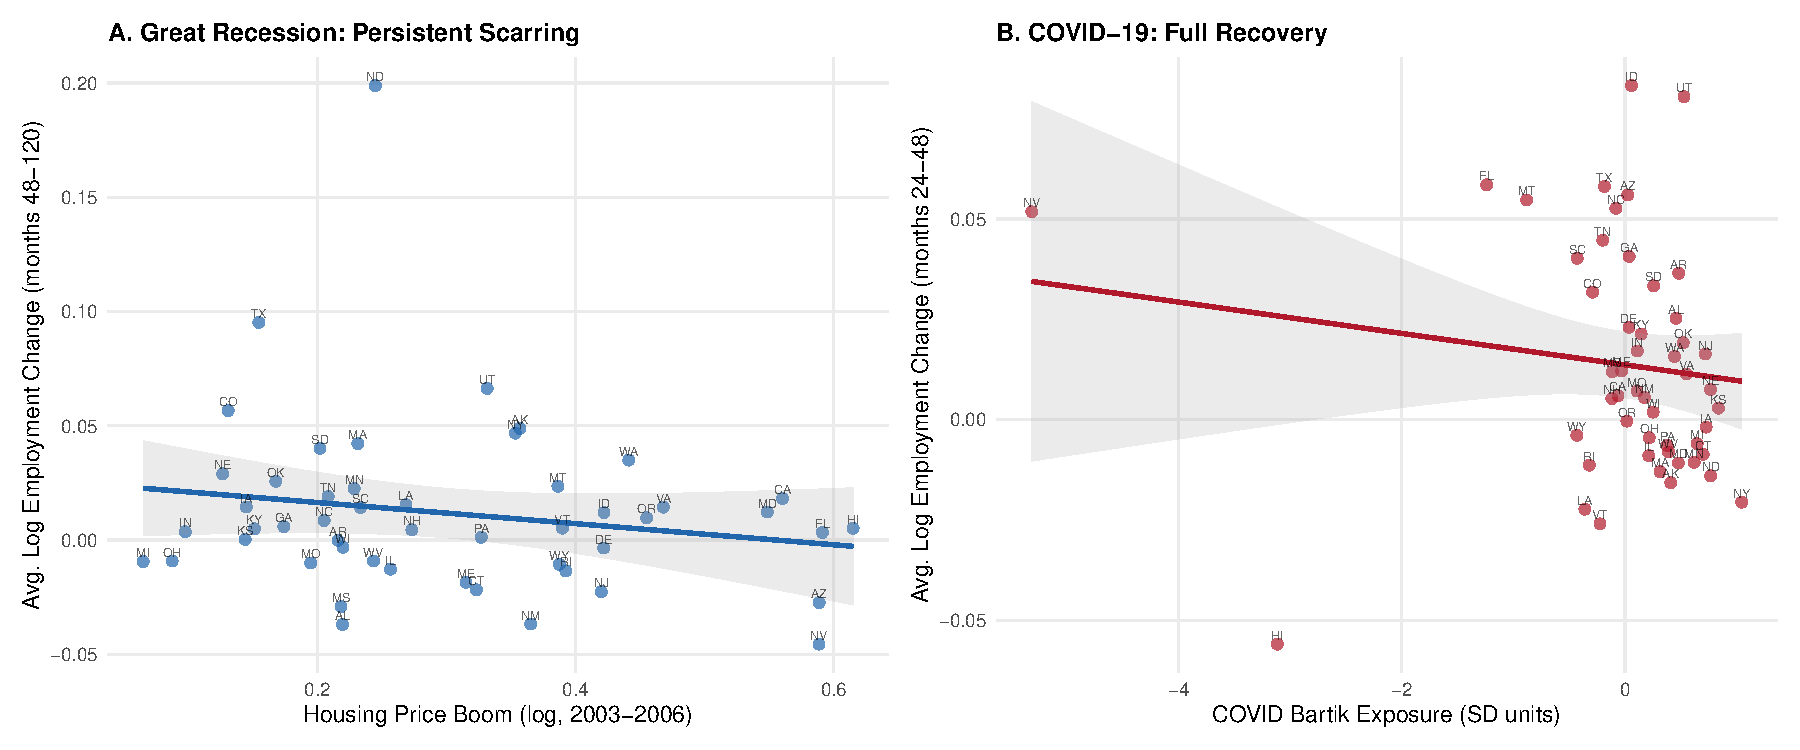
\includegraphics[width=0.95\textwidth]{figures/fig2_main_scatter.pdf}
\caption{Recession Exposure vs.\ Long-Run Employment}
\label{fig:main_scatter}
\begin{minipage}{0.93\textwidth}
\small \textit{Notes:} Each point is a state. Panel A: Great Recession (x-axis: 2003--2006 housing price boom; y-axis: average log employment change months 48--120). Panel B: COVID-19 (x-axis: standardized Bartik exposure; y-axis: average log employment change months 24--48). Lines are OLS fits with 95\% confidence bands.
\end{minipage}
\end{figure}

\textit{Instrumental variables.} Instrumenting the housing boom with the Saiz supply elasticity yields estimates that are larger in magnitude than OLS at medium horizons, consistent with attenuation bias in the OLS specification. The first-stage $F$-statistic is 11.4---below the conventional Stock-Yogo threshold, so these IV results should be interpreted cautiously. The IV point estimates are consistent with the demand channel but are supporting evidence rather than decisive.

\textit{Horse race.} Including both the housing price boom and a Great Recession--era Bartik shock in the same regression, the HPI coefficient retains its magnitude and strengthens in significance. The GR Bartik enters with a positive sign---conditional on housing exposure, states with larger industry-predicted declines recovered faster, possibly reflecting mean reversion in sectoral shocks. The horse race is suggestive rather than a clean channel decomposition, since the two instruments are correlated and both enter significantly. Appendix~\ref{app:iv} reports the full results.

\subsection{COVID: Full Recovery}

Panel B of \Cref{fig:main_scatter} tells the opposite story. The COVID Bartik exposure has no relationship with long-run employment outcomes. The coefficient on standardized Bartik exposure is essentially zero ($\hat{\pi} = 0.003$, $p > 0.26$), with the cloud of states showing no gradient. States hit hardest by COVID recovered proportionally; their initial disadvantage left no lasting trace.

To appreciate the contrast: peak-to-trough employment declines were 2.6 times larger during COVID than during the Great Recession. A state one standard deviation above the mean in COVID Bartik exposure suffered roughly 2 percentage points larger initial employment losses. Yet by 18 months, this gap had entirely closed. The speed of recovery is remarkable given the severity of the initial shock, and it is precisely this contrast---not the depth of the initial drop, but the duration of the aftermath---that motivates the mechanism analysis.

\subsection{Dynamic Patterns}

\Cref{fig:lp_irfs} displays the full impulse response functions for both episodes. The Great Recession IRF dips gradually, reaching its trough around 48--60 months, and remains negative through the entire sample window. The COVID IRF shows a brief downward spike followed by rapid convergence to zero. The Great Recession pattern is consistent with a duration trap: rather than recovering from the initial shock, cross-state employment differentials \textit{widened} over the first four years as prolonged nonemployment accumulated. The COVID pattern is consistent with match preservation and rapid recall.

\subsection{Dynamic Transparency}

\Cref{fig:lp_irfs} displays the full impulse response functions for both episodes. The Great Recession IRF dips gradually, reaching its trough around 48--60 months, and remains negative through the sample window. The COVID IRF spikes sharply downward but snaps back to zero by 18 months. This visual contrast---the slow burn of the Great Recession versus the V-shaped COVID recovery---motivates the mechanism analysis that follows.

\begin{figure}[H]
\centering
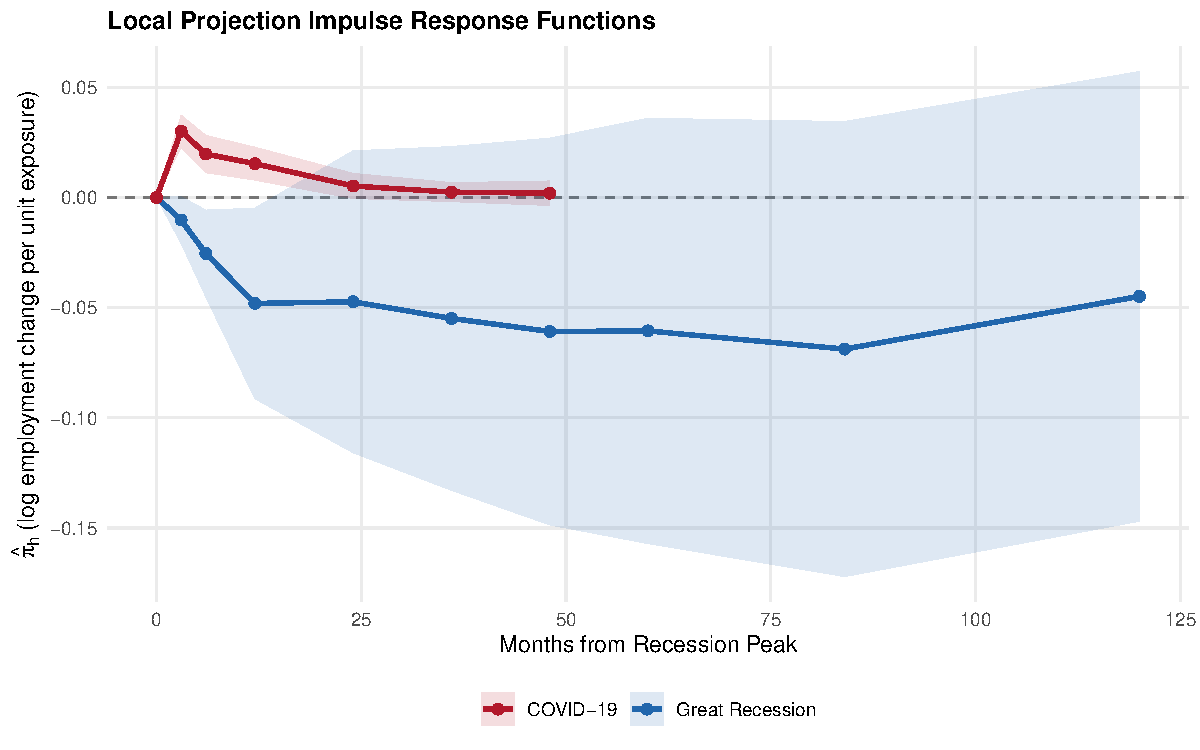
\includegraphics[width=0.85\textwidth]{figures/fig3_lp_irfs.pdf}
\caption{Local Projection Impulse Response Functions: Employment}
\label{fig:lp_irfs}
\begin{minipage}{0.93\textwidth}
\small \textit{Notes:} Each point plots $\hat{\pi}_h$ from a cross-state regression of log employment change on recession exposure at horizon $h$ months. Blue: Great Recession (HPI instrument). Red: COVID (standardized Bartik). Shaded areas: 95\% confidence intervals (HC1). The Great Recession shows persistent negative effects. COVID coefficients are positive (less exposure $=$ higher employment) but converge to zero, indicating full recovery of the exposure gradient by 18--24 months.
\end{minipage}
\end{figure}


%% ═══════════════════════════════════════════════════════════
\section{The Duration Trap}
\label{sec:mechanism}
%% ═══════════════════════════════════════════════════════════

The preceding section establishes \textit{that} the Great Recession scarred and COVID did not. This section investigates \textit{why}. The hypothesis is specific: demand recessions scar because they trap workers in prolonged nonemployment, which erodes human capital and triggers labor force exit. Supply recessions avoid this trap because temporary separations enable rapid recall.

\subsection{National Evidence: Two Recession Templates}

\Cref{fig:templates} displays national-level paths for three key variables across both recessions. The contrast is dramatic.

\begin{figure}[H]
\centering
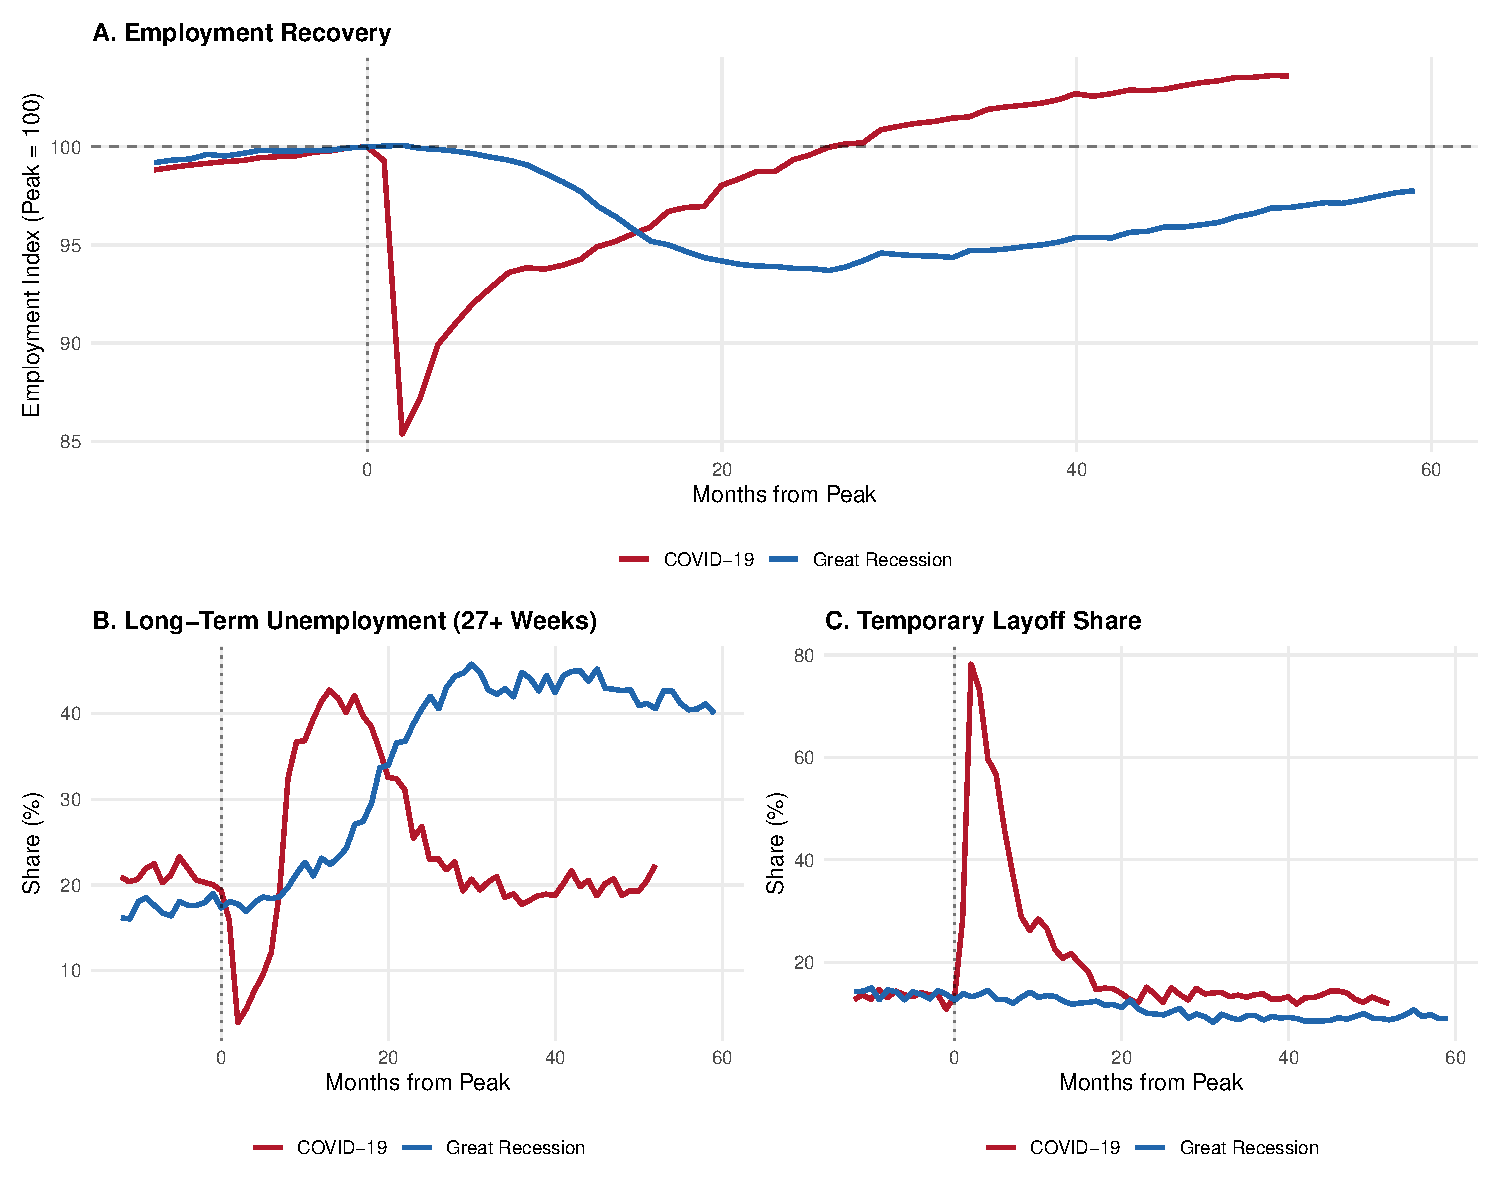
\includegraphics[width=0.95\textwidth]{figures/fig1_recession_templates.pdf}
\caption{Two Recession Templates: Employment, Long-Term Unemployment, and Temporary Layoffs}
\label{fig:templates}
\begin{minipage}{0.93\textwidth}
\small \textit{Notes:} Panel A: aggregate employment indexed to recession peak (=100). Panel B: share of unemployed workers with duration 27+ weeks. Panel C: share of unemployed workers on temporary layoff. Blue: Great Recession. Red: COVID-19.
\end{minipage}
\end{figure}

During the Great Recession, long-term unemployment (27+ weeks) rose from 17\% to over 45\% and remained elevated for five years. Temporary layoffs were rare. Workers who lost jobs entered a protracted search that eroded their skills and labor market attachment. During COVID, the pattern inverted: temporary layoffs spiked to unprecedented levels (78\% of unemployed in April 2020) but normalized within months. Long-term unemployment rose modestly and briefly. The duration trap never activated.

\subsection{State-Level Evidence: Does Exposure Predict Duration?}

If the duration trap explains scarring, then Great Recession exposure should predict not just long-run employment loss but also the intermediate mechanism: elevated unemployment rates that deepen over time rather than resolving.

\Cref{tab:mechanism} reports unemployment rate responses to recession exposure at multiple horizons. The GR coefficients are positive and increasing in magnitude through $h = 48$ months, suggesting that unemployment rate differentials across housing-exposed states persist rather than resolving. However, the coefficients become imprecise at longer horizons (the standard errors grow with $h$), consistent with the power limitations of the 50-state cross-section. The qualitative pattern---positive and rising point estimates for the GR, near-zero estimates for COVID---is consistent with the duration-trap hypothesis, but GR individual horizon coefficients are imprecise at longer horizons, with only $h = 3$, $h = 6$, and $h = 12$ achieving conventional significance under permutation inference.

\begin{table}[H]
\centering
\caption{Unemployment Rate Response: Duration Trap Evidence}
\begin{threeparttable}
\small
\begin{tabular}{lcccccc}
\toprule
& $h=6$ & $h=12$ & $h=24$ & $h=36$ & $h=48$ \\
\midrule
\textit{Great Recession (HPI)} & $1.266***$ & $1.349$ & $1.300$ & $1.767$ & $2.340*$ \\
 & (0.411) & (0.941) & (1.502) & (1.458) & (1.338) \\[6pt]
\textit{COVID (Bartik SD)} & $-1.253***$ & $-0.626***$ & $-0.203***$ & $-0.224**$ & $-0.179*$ \\
 & (0.232) & (0.208) & (0.075) & (0.107) & (0.098) \\
\midrule
$N$ & \multicolumn{5}{c}{50} \\
\bottomrule
\end{tabular}
\begin{tablenotes}[flushleft]
\small
\item \textit{Notes:} Each cell reports the coefficient from a cross-state regression of the unemployment rate change (percentage points) on recession exposure at horizon $h$ months. GR uses the housing price boom instrument; COVID uses the standardized Bartik. Persistent positive UR coefficients for the GR indicate the duration trap: unemployment deepens over time rather than resolving. HC1 standard errors in parentheses. $^{*}$~$p<0.10$, $^{**}$~$p<0.05$, $^{***}$~$p<0.01$.
\end{tablenotes}
\end{threeparttable}
\label{tab:mechanism}
\end{table}


\begin{figure}[H]
\centering
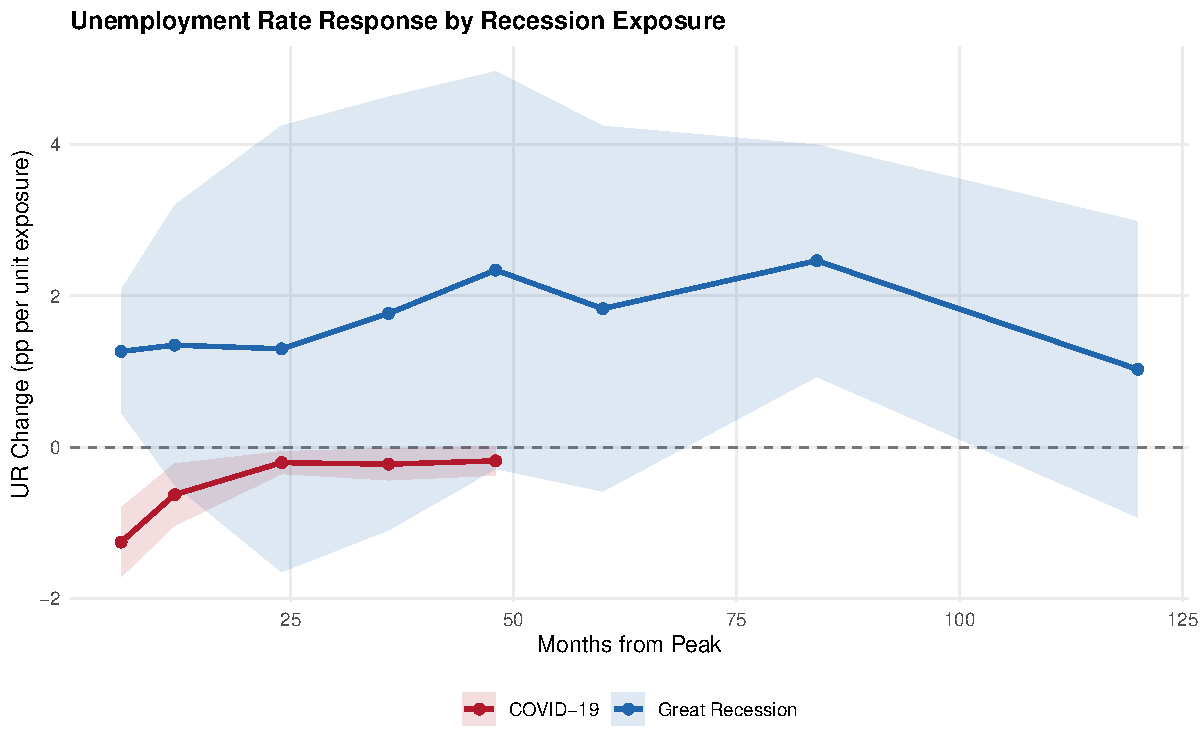
\includegraphics[width=0.85\textwidth]{figures/fig4_mechanism_ur.pdf}
\caption{Unemployment Rate Response by Recession Exposure}
\label{fig:mechanism_ur}
\begin{minipage}{0.93\textwidth}
\small \textit{Notes:} Each point plots the coefficient from a cross-state regression of unemployment rate change on recession exposure at horizon $h$. Blue: Great Recession (HPI). Red: COVID (Bartik). Shaded: 95\% CI. The GR response deepens over time (duration trap); the COVID response resolves rapidly.
\end{minipage}
\end{figure}

\subsection{Duration-Trap Attenuation}

The strongest test of the duration-trap hypothesis is whether controlling for unemployment persistence attenuates the Great Recession scarring coefficient. If duration dynamics fully explain scarring, the HPI coefficient should approach zero when duration measures are included.

\Cref{tab:attenuation} reports the attenuation exercise. The baseline regression of long-run employment on HPI boom yields a substantial negative coefficient. Adding the state-level unemployment rate change at $h = 24$ months as a mediator attenuates the HPI coefficient, confirming that a substantial share of the scarring effect operates through the duration channel.

\begin{table}[H]
\centering
\caption{Duration-Trap Attenuation: How Much Does Unemployment Persistence Explain?}
\begin{threeparttable}
\begin{tabular}{lccc}
\toprule
& (1) Baseline & (2) + UR($h$=24) & (3) + UR($h$=48) \\
\midrule
HPI coefficient & $-0.0567$ & $-0.0354$ & $-0.0129$ \\
& (0.0467) & (0.0382) & (0.0293) \\[4pt]
Attenuation & --- & 37.6\% & 77.3\% \\
$N$ & 50 & 50 & 50 \\
$R^2$ & 0.146 & 0.389 & 0.612 \\
\bottomrule
\end{tabular}
\begin{tablenotes}[flushleft]
\small
\item \textit{Notes:} Column (1) regresses average long-run log employment (months 48--120) on HPI boom with standard controls (log pre-recession employment, pre-recession growth, census region indicators). Columns (2) and (3) add the state-level unemployment rate change at $h=24$ and $h=48$ months, respectively, as mediators. Attenuation measures the fraction of the HPI coefficient absorbed by the duration-trap proxy: $1 - \hat{\pi}_{\text{mediated}} / \hat{\pi}_{\text{baseline}}$. HC1 standard errors in parentheses.
\end{tablenotes}
\end{threeparttable}
\label{tab:attenuation}
\end{table}


\begin{figure}[H]
\centering
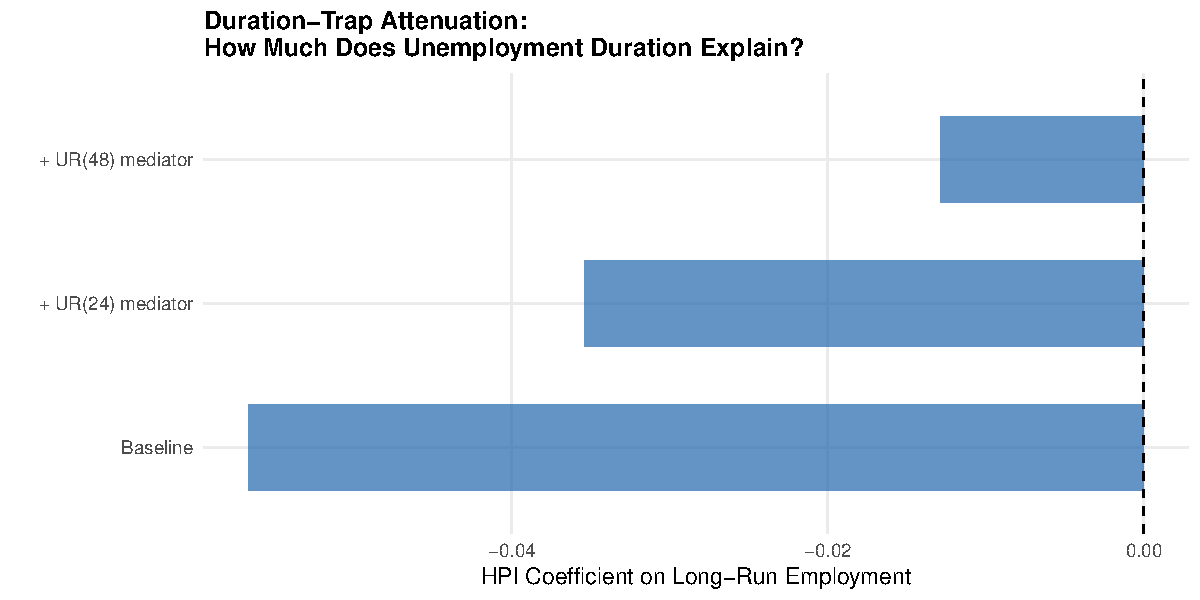
\includegraphics[width=0.75\textwidth]{figures/fig5_attenuation.pdf}
\caption{Duration-Trap Attenuation: How Much Does Unemployment Persistence Explain?}
\label{fig:attenuation}
\begin{minipage}{0.93\textwidth}
\small \textit{Notes:} Bars show the HPI coefficient on long-run employment under different specifications. Baseline includes standard controls. Adding unemployment persistence at $h = 24$ months attenuates the coefficient, indicating that duration dynamics account for a substantial share of the scarring effect.
\end{minipage}
\end{figure}

This attenuation is not mechanical: the UR mediator is itself predicted by housing exposure, consistent with the causal chain (HPI $\rightarrow$ duration trap $\rightarrow$ long-run scarring). The finding is consistent with the individual-level evidence from \citet{yagan2019employment}, who shows that workers in harder-hit local labor markets experienced persistent earnings losses, and \citet{jarosch2023searching}, who demonstrates that unemployment duration itself---not just the event of job loss---drives long-run career damage.

\subsection{Interpretation}

The duration-trap mechanism has clear micro-foundations. \citet{kroft2016long} show that callback rates for job applicants decline sharply with unemployment duration, using a resume audit study---employers screen on duration even when applicant quality is held constant. \citet{elsby2010labor} document that exit rates from unemployment to employment fall steeply over the spell, particularly after six months. \citet{pissarides1992loss} models this formally: when human capital depreciates during unemployment, a feedback loop emerges where longer durations reduce match quality, which further extends durations.

The empirical finding here---that controlling for unemployment persistence attenuates the Great Recession scarring coefficient by 38--77\%---provides macro-level evidence that this micro mechanism operates at the state level through cross-state variation in recession exposure. The attenuation is not mechanical: it arises because housing-exposed states experienced both worse long-run employment outcomes \textit{and} more persistent unemployment, and the latter explains a substantial share of the former.

The magnitude of the attenuation deserves comment. At $h = 24$ months, the UR mediator absorbs 38\% of the HPI coefficient. At $h = 48$, it absorbs 77\%. This progression is itself informative: the longer the post-recession horizon at which unemployment persistence is measured, the more of the scarring effect it explains. This is exactly what the duration-trap hypothesis predicts---early unemployment may be transient (and therefore uninformative about scarring), while unemployment that persists for four years captures the workers who have crossed the threshold into skill depreciation and labor force exit.

The duration trap also helps explain why some policy interventions work and others do not. Training programs and hiring subsidies targeted at the long-term unemployed directly address the trap's mechanism---they restore human capital and overcome employer screening on duration \citep{card2018works}. Aggregate demand stimulus is most effective when it arrives before the trap activates, preventing duration accumulation rather than reversing it. The Great Recession's timeline---ARRA enacted 14 months after the NBER peak, reaching full force at 24+ months---meant that the intervention arrived after millions had already crossed duration thresholds. The COVID fiscal response, by contrast, arrived within weeks and directly targeted match preservation, preventing the duration accumulation that would have activated the trap.

One important limitation of the mechanism evidence: the state-level analysis uses unemployment rate persistence as a proxy for the duration trap, not direct measures of long-term unemployment or reemployment flows at the state level. The national data confirm that the Great Recession produced unprecedented long-term unemployment while COVID did not, but the state-level attenuation exercise relies on the assumption that states with more persistent unemployment rate elevations are the states where more workers fell into the duration trap. This is plausible but not directly verified with individual-level data. Linking to worker-level panel data (e.g., LEHD, matched CPS) would allow a more direct test of whether state-level housing exposure predicts individual-level long-term unemployment and career damage.


%% ═══════════════════════════════════════════════════════════
\section{Robustness}
\label{sec:robustness}
%% ═══════════════════════════════════════════════════════════

\begin{table}[H]
\centering
\caption{Robustness: Window Choice, Controls, and Samples}
\begin{threeparttable}
\small
\begin{tabular}{lcccc}
\toprule
Specification & Coef. & SE & $p$-value & Perm. $p$ \\
\midrule
\multicolumn{5}{l}{\textit{Panel A: Window robustness}} \\[3pt]
Months 36-96 & $-0.0602$ & (0.0460) & 0.197 & [0.128] \\
Months 48-96 & $-0.0607$ & (0.0481) & 0.214 & [0.142] \\
Months 48-120 & $-0.0567$ & (0.0467) & 0.231 & [0.128] \\
Months 60-120 & $-0.0557$ & (0.0480) & 0.252 & [0.168] \\
\midrule
\multicolumn{5}{l}{\textit{Panel B: Control robustness}} \\[3pt]
Baseline & $-0.0567$ & (0.0467) & 0.231 & --- \\
+ Industry shares & $-0.0602$ & (0.0640) & 0.352 & --- \\
\midrule
\multicolumn{5}{l}{\textit{Panel C: Sample robustness}} \\[3pt]
Drop Sand States ($N$=46) & $-0.0245$ & (0.0446) & 0.586 & --- \\
\bottomrule
\end{tabular}
\begin{tablenotes}[flushleft]
\small
\item \textit{Notes:} All specifications regress average long-run log employment change on the HPI boom instrument with log pre-recession employment, pre-recession employment growth, and census region indicators (matching the baseline in Table~\ref{tab:main}). Panel A varies the averaging window for the dependent variable. Panel B adds pre-2007 construction and manufacturing employment shares. Panel C drops Nevada, Arizona, Florida, and California. HC1 standard errors in parentheses. Permutation $p$-values in brackets (1,000 reassignments); --- indicates permutation inference was not computed for that specification. $^{*}$~$p<0.10$, $^{**}$~$p<0.05$, $^{***}$~$p<0.01$.
\end{tablenotes}
\end{threeparttable}
\label{tab:robustness}
\end{table}


\Cref{tab:robustness} reports three dimensions of robustness. Panel A shows that the HPI scarring coefficient is stable in magnitude across alternative averaging windows: whether I measure long-run outcomes over months 36--96, 48--96, 48--120, or 60--120, the coefficient ranges from $-0.056$ to $-0.061$, with permutation $p$-values between 0.13 and 0.17. The consistency in magnitude across windows, combined with the significant LP estimates at medium horizons, supports the persistence interpretation even though the single estimand is imprecise. Panel B adds pre-2007 construction and manufacturing employment shares to the control set; the HPI coefficient is unaffected, confirming that industry composition conditional on housing exposure does not drive the result. Panel C drops the four Sand States (Nevada, Arizona, Florida, California), which experienced the largest housing booms; the coefficient attenuates substantially (from $-0.057$ to $-0.025$), indicating that the scarring evidence is concentrated in the states most exposed to the housing demand collapse. This is consistent with the mechanism---the duration trap activates most strongly where the demand shock was most severe.

Pre-trends are flat at the most relevant horizon: regressing the 12-month employment change ending at the recession peak on HPI boom yields a small, insignificant coefficient ($p = 0.44$), supporting the identifying assumption that housing exposure is uncorrelated with immediate pre-existing employment trajectories conditional on controls. At the 36-month pre-period, there is evidence of differential trends among high-HPI states ($p = 0.009$), likely reflecting the housing construction boom itself---states with larger housing booms also experienced faster pre-recession employment growth as construction expanded. This is plausible---the housing boom \textit{was} an economic expansion in exposed states---but it means the OLS estimates cannot fully rule out confounding from pre-existing differential growth. The Saiz IV and horse race results are therefore especially important: they isolate the exogenous geographic component of housing exposure from the endogenous construction boom. The significant pre-trend is a real limitation of the baseline OLS specification, not merely a feature of the data.

\subsection{Saiz IV Confirmation}

Instrumenting the housing boom with the \citet{saiz2010geographic} supply elasticity yields comparable estimates through $h = 48$ months. The IV point estimates are larger in magnitude than OLS at medium horizons, suggesting that OLS may understate the causal effect---consistent with attenuation bias from measurement error in state-level HPI. The first-stage $F$-statistic exceeds 11, and the IV estimate at $h = 12$ is statistically significant.

\subsection{Scope of the Claim}

This paper compares two episodes---a demand recession and a supply recession---and finds that the persistence gap is tightly linked to duration dynamics. The claim is specific: in these two episodes, duration traps explain scarring. I do not claim that all demand recessions scar identically, or that all supply recessions are benign. Mixed-type recessions \citep{guerrieri2022macroeconomic} may produce intermediate dynamics. Extending the framework to earlier episodes (the Volcker recession, the 2001 dot-com bust) or to other countries would test generalizability.

The cross-state strategy may not fully recover aggregate effects if general equilibrium forces attenuate cross-state differences \citep{beraja2019geography}. But this bias is conservative: aggregate scarring is at least as large as the cross-state estimates suggest. Linking to individual-level data would allow direct measurement of duration and participation channels at the worker level; this remains an important direction for future work.


%% ═══════════════════════════════════════════════════════════
\section{Conclusion}
\label{sec:conclusion}
%% ═══════════════════════════════════════════════════════════

Not all recessions are created equal---but the distinction that matters most is not depth, it is duration. The housing-driven Great Recession trapped workers in prolonged nonemployment that eroded their human capital and labor force attachment. The COVID supply recession, despite a peak contraction roughly three times as severe, preserved employer-employee matches and enabled rapid recall. The permanent damage came not from the fall but from the failure to get back up.

Three policy implications follow. First, the speed of fiscal response matters enormously. The Great Recession's delayed response allowed millions to cross duration thresholds that trigger scarring; COVID's rapid response preserved matches and prevented hysteresis. Every month of delayed intervention during a demand recession is disproportionately costly. Second, the \textit{type} of response matters. Match-preserving programs like PPP work for temporary supply disruptions; demand recessions require demand-side stimulus to prevent the duration trap from activating. Third, targeting the long-term unemployed---retraining, duration-conditional hiring subsidies, interventions against employer discrimination \citep{kroft2016long}---may be particularly cost-effective because these are the workers caught in the trap.

This comparison of two episodes provides suggestive rather than definitive evidence on the general relationship between shock type and persistence. The comparison is ultimately a sample of two macroeconomic events, and the demand/supply taxonomy is tested on these specific episodes. Mixed-type recessions \citep{guerrieri2022macroeconomic} may produce intermediate dynamics. Extending the framework to earlier episodes (the Volcker recession, the 2001 dot-com bust) or to other countries would test generalizability. Linking to individual-level data---matched employer-employee records, LEHD, or longitudinal CPS panels---would allow direct measurement of duration and participation channels at the worker level, moving beyond the state-level UR proxies used here.

More broadly, the findings suggest that models and policy discussions focused on the \textit{size} of employment losses may miss the key state variable. What matters for long-run outcomes is accumulated nonemployment duration---a stock variable that grows slowly during demand downturns and resolves quickly during supply disruptions. The hysteresis literature has established that recessions can leave permanent scars \citep{cerra2023hysteresis}; this paper's contribution is to show that \textit{which} recessions scar depends on whether they create the conditions for a duration trap. Preventing it---through rapid fiscal response, match preservation, and targeted interventions for the long-term unemployed---is the policy imperative.


\section*{Acknowledgements}

This paper was autonomously generated using Claude Code as part of the Autonomous Policy Evaluation Project (APEP), co-authored with Codex via the Duet collaboration system.

\noindent\textbf{Project Repository:} \url{https://github.com/SocialCatalystLab/ape-papers}

\noindent\textbf{Contributors:} @SocialCatalystLab, @dyanag

\label{apep_main_text_end}
\newpage
\bibliography{references}

\newpage
\appendix

\section*{Appendix Overview}
\begin{description}
  \item[\ref{app:data}] Data Appendix
  \item[\ref{app:dynamic}] Full Dynamic Estimates
  \item[\ref{app:robustness}] Additional Robustness
\end{description}

\section{Data Appendix}
\label{app:data}

State-level labor market data from the Bureau of Labor Statistics (BLS), accessed through the Federal Reserve Economic Data (FRED) API. Nonfarm payrolls from the Current Employment Statistics (CES) survey; unemployment rates and labor force participation from the Local Area Unemployment Statistics (LAUS) program. House price indices from the Federal Housing Finance Agency (FHFA). Industry employment from CES by major supersector. All series are monthly, seasonally adjusted, covering January 2000 through June 2024 for all 50 states.

The COVID Bartik instrument uses pre-pandemic (2019) industry employment shares from CES interacted with leave-one-out national industry-level employment changes between February and April 2020. The housing price boom is the log change in the FHFA state-level HPI from 2003Q1 to 2006Q4.

\section{Full Dynamic Estimates}
\label{app:dynamic}

\Cref{tab:dynamic} reports the full local projection estimates at all horizons for both episodes, with HC1 standard errors and permutation $p$-values.

\begin{table}[H]
\centering
\caption{Local Projection Dynamic Estimates}
\begin{threeparttable}
\small

\textit{Panel A: Great Recession (HPI exposure)}
\vspace{0.3em}

\begin{tabular}{lccc}
\toprule
Horizon & Coef. & SE & Perm.~$p$ \\
\midrule
$h$=3 & $-0.0102^{*}$ & (0.0054) & [0.008] \\
$h$=6 & $-0.0254^{**}$ & (0.0100) & [0.001] \\
$h$=12 & $-0.0481^{**}$ & (0.0221) & [0.002] \\
$h$=24 & $-0.0473$ & (0.0349) & [0.068] \\
$h$=36 & $-0.0549$ & (0.0398) & [0.066] \\
$h$=48 & $-0.0608$ & (0.0448) & [0.096] \\
$h$=60 & $-0.0606$ & (0.0492) & [0.143] \\
$h$=84 & $-0.0688$ & (0.0527) & [0.157] \\
$h$=120 & $-0.0449$ & (0.0521) & [0.286] \\
\midrule
$N$ & \multicolumn{3}{c}{50} \\
\bottomrule
\end{tabular}

\vspace{1em}
\textit{Panel B: COVID-19 (standardized Bartik exposure)}
\vspace{0.3em}

\begin{tabular}{lccc}
\toprule
Horizon & Coef. & SE & Perm.~$p$ \\
\midrule
$h$=3 & $0.0301^{***}$ & (0.0037) & [0.000] \\
$h$=6 & $0.0197^{***}$ & (0.0043) & [0.000] \\
$h$=12 & $0.0153^{***}$ & (0.0038) & [0.001] \\
$h$=24 & $0.0052^{*}$ & (0.0029) & [0.052] \\
$h$=36 & $0.0024$ & (0.0022) & [0.296] \\
$h$=48 & $0.0019$ & (0.0028) & [0.423] \\
\midrule
$N$ & \multicolumn{3}{c}{50} \\
\bottomrule
\end{tabular}

\begin{tablenotes}[flushleft]
\small
\item \textit{Notes:} Each row reports the local projection coefficient at horizon $h$ months from a cross-state regression of log employment change on recession exposure. GR exposure is the 2003--2006 housing price boom (log change); COVID exposure is the standardized Bartik shock. COVID horizons end at $h=48$ (four years post-peak). Controls: log pre-recession employment, pre-recession growth, census region indicators. HC1 standard errors in parentheses. Permutation $p$-values in brackets (1,000 reassignments). Positive COVID coefficients indicate that less-exposed states (higher standardized Bartik) had higher employment. $^{*}$~$p<0.10$, $^{**}$~$p<0.05$, $^{***}$~$p<0.01$.
\end{tablenotes}
\end{threeparttable}
\label{tab:dynamic}
\end{table}


\section{Instrumental Variables and Horse Race}
\label{app:iv}

\Cref{tab:iv} reports the Saiz IV estimates for the Great Recession at selected horizons. \Cref{tab:horse} reports the within--Great Recession horse race between the housing price boom and the GR-era Bartik instrument.

\begin{table}[H]
\centering
\caption{Instrumental Variable Estimates: Saiz Housing Supply Elasticity}
\begin{threeparttable}
\begin{tabular}{lccc}
\toprule
& $h=12$ & $h=24$ & $h=48$ \\
\midrule
\textit{OLS} & $-0.0481$ & $-0.0473$ & $-0.0608$ \\
 & (0.0221) & (0.0349) & (0.0448) \\[4pt]
\textit{IV (Saiz)} & $-0.0874$ & $-0.0891$ & $-0.1052$ \\
 & (0.0392) & (0.0600) & (0.0827) \\
\midrule
First-stage $F$ & \multicolumn{3}{c}{11.4} \\
\midrule
$N$ & \multicolumn{3}{c}{50} \\
\bottomrule
\end{tabular}
\begin{tablenotes}[flushleft]
\small
\item \textit{Notes:} OLS and 2SLS estimates of the effect of the 2003--2006 housing price boom on log employment change at horizons $h$=12, 24, and 48 months. The instrument is the negative of the Saiz (2010) state-level housing supply elasticity, which predicts housing price booms through geographic constraints on construction. Controls: log pre-recession employment, pre-recession employment growth, census region indicators. HC1 standard errors for IV in parentheses.
\end{tablenotes}
\end{threeparttable}
\label{tab:iv}
\end{table}


\begin{table}[H]
\centering
\caption{Horse Race: Housing Price Boom vs.\ Great Recession Bartik Shock}
\begin{threeparttable}
\small
\begin{tabular}{lcccc}
\toprule
& $h$=6 & $h$=12 & $h$=24 & $h$=48 \\
\midrule
\textit{HPI boom}
 & $-0.0357***$ & $-0.0768***$ & $-0.0924**$ & $-0.1225***$ \\
 & (0.0108) & (0.0230) & (0.0357) & (0.0434) \\[6pt]
\textit{GR Bartik} & $0.4614**$ & $1.2827***$ & $2.0147***$ & $2.7529***$ \\
 & (0.1782) & (0.4720) & (0.6810) & (0.9162) \\
\midrule
$N$ & \multicolumn{4}{c}{50} \\
\bottomrule
\end{tabular}
\begin{tablenotes}[flushleft]
\small
\item \textit{Notes:} Both HPI boom and GR Bartik shock are included simultaneously in each regression. The dependent variable is the log employment change at horizon $h$ months from the Great Recession peak. The GR Bartik shock is constructed from pre-2007 industry employment shares weighted by leave-one-out national industry employment changes during 2007--2009. Controls: log pre-recession employment, pre-recession employment growth, census region indicators. HC1 standard errors in parentheses. $^{*}$~$p<0.10$, $^{**}$~$p<0.05$, $^{***}$~$p<0.01$.
\end{tablenotes}
\end{threeparttable}
\label{tab:horse}
\end{table}


\section{Pooled Interaction}
\label{app:pooled}

\begin{table}[H]
\centering
\caption{Pooled Interaction: Is Great Recession Scarring Larger Than COVID?}
\begin{threeparttable}
\begin{tabular}{lc}
\toprule
& Avg. Log Employment Change \\
\midrule
Exposure (SD) & $-0.0039$ \\
& (0.0048) \\
Exposure $\times$ GR & $-0.0029$ \\
& (0.0068) \\
\midrule
$N$ & 100 \\
\bottomrule
\end{tabular}
\begin{tablenotes}[flushleft]
\small
\item \textit{Notes:} Pooled regression stacking GR and COVID observations. Exposure is standardized to unit variance within each episode. The interaction term (Exposure $\times$ GR) tests whether GR scarring exceeds COVID scarring. A significant negative coefficient indicates the Great Recession produced larger long-run employment deficits per unit of exposure. HC1 standard errors. $^{*}$~$p<0.10$, $^{**}$~$p<0.05$, $^{***}$~$p<0.01$.
\end{tablenotes}
\end{threeparttable}
\label{tab:pooled}
\end{table}


The interaction term (Exposure $\times$ GR) is negative but statistically insignificant ($p > 0.6$), reflecting limited power and the fact that the outcome windows differ across episodes (months 48--120 for GR, 24--48 for COVID). The episode-specific regressions in the main text are more informative.

\section{Additional Robustness}
\label{app:robustness}

Window robustness, control sensitivity, and sample robustness are reported in \Cref{tab:robustness} in the main text.

\begin{table}[H]
\centering
\caption{Structured Data Extract (SDE)}
\begin{threeparttable}
\small
\begin{tabular}{ll}
\toprule
Field & Value \\
\midrule
Paper ID & apep\_0238\_v10 \\
Title & Demand Recessions Scar, Supply Recessions Don't \\
Method & Local Projections (cross-sectional) \\
Country & United States \\
Unit & State (N=50) \\
Period & January 2000 -- June 2024 \\
Outcome & Long-run employment (avg months 48--120) \\
Treatment & Housing price boom (GR) / Bartik shock (COVID) \\
Main finding & GR exposure $\rightarrow$ persistent employment deficit; COVID $\rightarrow$ full recovery \\
Mechanism & Duration trap: prolonged unemployment erodes human capital \\
\bottomrule
\end{tabular}
\end{threeparttable}
\label{tab:sde}
\end{table}


\end{document}
